\clearpage
\begingroup
\emergencystretch=1em
\section{Experiment P2E: IMU sensitivity of the communication curve}
\label{sec:p2e}
\subsection{Question and frozen design}
P2A--P2D used one IMU quality setting. P2E asks how white sensor noise and slowly varying bias change the UWB effort needed to preserve relative localization accuracy. It also separates sensitivity of the existing estimator from a limited process-noise adjustment. Sensor quality is varied while the four paths, \SI{60}{s} duration, \SI{100}{Hz} sampling, known initial positions/headings, initial-velocity uncertainty, Gaussian range noise, and 20 seeds remain fixed.

Cyclic is the scheduling reference. The budgets are \(B\in\{0,180,360,720,3600\}\), corresponding to 0\%, 5\%, 10\%, 20\%, and 100\% of full communication. Positive budgets use the P2C allocation in Eq.~\ref{eq:p2c_capacity}. At 3600, every \SI{10}{Hz} opportunity activates all six pairs, recovering the P2A full-range schedule. Intermediate budgets retain P2C timing, rather than P2B's simultaneous all-link rounds. Ranges remain clean Gaussian with \(\sigma_r=\SI{0.12}{m}\); every attempted exchange is received and accepted. There is no innovation gate or global reference in P2E.

Table~\ref{tab:p2e_conditions} specifies the six conditions, frozen before evaluation. White multipliers scale both accelerometer and gyroscope per-sample standard deviations. Bias multipliers scale both random-walk diffusion amplitudes, not their variances. Reference white standard deviations are \SI{0.02}{m/s^2} and \SI{0.001}{rad/s}; reference bias diffusion amplitudes are \(5\times10^{-5}\)~\(\mathrm{m\,s^{-2}/\sqrt{s}}\) and \(5\times10^{-6}\)~\(\mathrm{rad\,s^{-1}/\sqrt{s}}\). Bias starts at zero. Initial constant offsets are not introduced, and the \SI{0.05}{m/s} initial-velocity error standard deviation is retained even for improved sensors.
\begin{table}[htbp]
\centering
\caption{Predefined P2E sensor conditions. Multipliers apply jointly to accelerometer and gyroscope; they are controlled sensitivity levels, not hardware quality grades.}
\label{tab:p2e_conditions}
\begin{tabular}{lrr}
\toprule
Condition & White amplitude & Bias diffusion amplitude \\
\midrule
Reference & 1 & 1 \\
White noise $\times0.5$ & 0.5 & 1 \\
White noise $\times4$ & 4 & 1 \\
Bias drift $\times0.5$ & 1 & 0.5 \\
Bias drift $\times10$ & 1 & 10 \\
Combined degraded & 4 & 10 \\
\bottomrule
\end{tabular}
\end{table}

For each seed and node, one reference realization is decomposed into ideal IMU, random-walk bias, and white noise. The same latent components are scaled separately across conditions. Reference measurements remain byte-identical to P2A. Range noise and initial-velocity errors are also shared across conditions and budgets. Thus seed comparisons change amplitudes without changing the underlying disturbance paths. Acceleration and gyroscope quality change together; P2E does not isolate their separate contributions.

\subsection{Fixed versus white-noise-rescaled process covariance}
The primary six-condition sweep freezes the EKF process standard deviations at \SI{0.03}{m/s^2} and \SI{0.0015}{rad/s}. It measures degradation of the existing estimator under changed sensor quality, including resulting process-noise mismatch.

A companion sweep uses identical measurements and schedules for the white-noise-half, white-noise-fourfold, and combined-degraded conditions. It multiplies both process standard deviations by the white amplitude multiplier, preserving the reference ratio of 1.5 between process and sensor white amplitudes. The existing covariance construction and its time-step powers are retained. This is labeled \emph{white-noise-rescaled \(Q\)}, not a fully calibrated filter. In particular, the five-state EKF has no bias states and does not model the temporally correlated bias random walk, including in the combined-degraded companion.

The primary sweep contains \(6\times5\times20=600\) runs; the companion adds \(3\times5\times20=300\), for 900 total. Each run checks communication accounting and squared fleet-error decomposition. All 100 reference-condition endpoints (five budgets, 20 seeds) reproduce committed P2C cyclic or P2B zero/full metrics within \(10^{-10}\) numerical tolerance. All 60 companion zero-UWB trajectories exactly equal their corresponding fixed-\(Q\) trajectories; changing covariance without range updates does not change inertial propagation.

Whole-run fleet, worst-node, centroid, relative-shape, yaw, and per-node RMSE use native \SI{100}{Hz} histories. Shape subtracts mean fleet position error without rotational alignment. Compact time profiles sample \SI{2}{Hz}; bands show pointwise mean \(\pm\) sample standard deviation, clipped at zero. Paired differences use 30,000 matched-seed bootstrap resamples and descriptive percentile 95\% intervals, unadjusted for multiple comparisons.

A descriptive \SI{0.10}{m} mean whole-run shape-RMSE target is also fixed before the campaign. We report the smallest \emph{tested} budget meeting it, with no interpolation. Empirical 95th percentiles and counts of passing seeds indicate variability; neither is a deployment guarantee or confidence bound from these 20 fixed-path realizations.

\subsection{Primary sensitivity results}
Table~\ref{tab:p2e_shape} summarizes mean shape RMSE across all budgets. Figure~\ref{fig:p2e_budget} separates relative shape from centroid and absolute position errors. The zero-UWB baseline is in the table; positive budgets use a logarithmic horizontal axis in the figure.
\begin{table}[htbp]
\centering\small
\caption{P2E fixed-\(Q\) mean whole-run relative-shape RMSE over 20 seeds, in metres. Budgets count individual undirected UWB exchanges. Variability and decomposition at 360 and 3600 exchanges are in Table~\ref{tab:p2e_decomposition}.}
\label{tab:p2e_shape}
\begin{tabular}{lrrrrr}
\toprule
Condition & 0 & 180 & 360 & 720 & 3600 \\
\midrule
Reference & 2.0273 & 0.1095 & 0.0824 & 0.0687 & 0.0456 \\
White noise $\times0.5$ & 1.9993 & 0.1040 & 0.0770 & 0.0637 & 0.0404 \\
White noise $\times4$ & 2.4313 & 0.1868 & 0.1569 & 0.1381 & 0.1096 \\
Bias drift $\times0.5$ & 2.0250 & 0.1088 & 0.0816 & 0.0681 & 0.0446 \\
Bias drift $\times10$ & 2.1874 & 0.1832 & 0.1562 & 0.1378 & 0.1119 \\
White $\times4$, bias $\times10$ & 2.5892 & 0.2382 & 0.2070 & 0.1850 & 0.1527 \\
\bottomrule
\end{tabular}
\end{table}

At 360 exchanges, reference shape RMSE is \SI{0.0824}{m}. Fourfold white noise increases it to \SI{0.1569}{m}; tenfold bias drift gives \SI{0.1562}{m}; combined degradation gives \SI{0.2070}{m}. Their paired increases over reference are respectively \(+0.07445\)~m (95\% interval \([0.06397,0.08545]\)~m), \(+0.07371\)~m (\([0.05727,0.09118]\)~m), and \(+0.12457\)~m (\([0.10022,0.15187]\)~m). All three conditions worsen shape RMSE in all 20 seeds at this budget.

More communication helps but does not eliminate the degradation. At 3600 exchanges, reference reaches \SI{0.0456}{m}, while fourfold white noise remains at \SI{0.1096}{m}, tenfold bias drift at \SI{0.1119}{m}, and combined degradation at \SI{0.1527}{m}. Even these full-budget degraded conditions are worse in mean shape accuracy than reference at 360 exchanges. This demonstrates a limit to substituting more ranging for sensor quality within the tested estimator, duration, and stress levels; it does not show that no alternative estimator could recover the target.

Halving white noise improves reference shape RMSE at 360 exchanges by \(-0.00544\)~m, interval \([-0.00716,-0.00378]\)~m, with 18/20 improvements. Halving bias drift changes it by only \(-0.00088\)~m, interval \([-0.00156,-0.00020]\)~m. The original bias level is already small over this run; reducing it further has a millimetre-scale effect, whereas increasing it tenfold reveals a substantial sensitivity. Known initial pose does not remove retained initial-velocity error or subsequent inertial drift.
\begin{figure}[htbp]
\centering
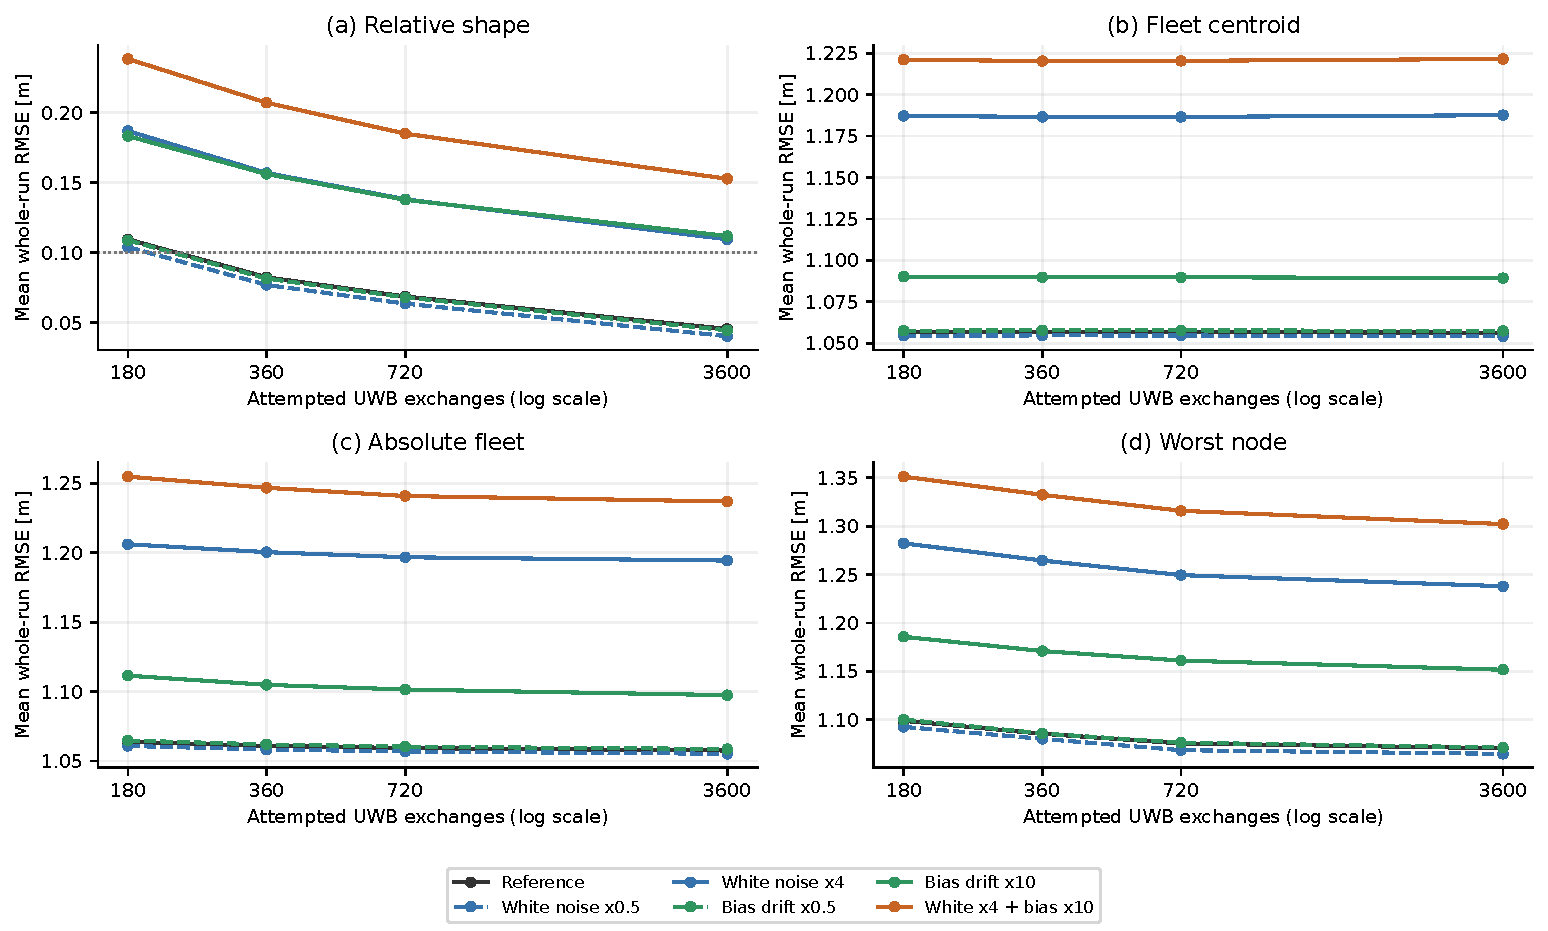
\includegraphics[width=\textwidth]{figures/phase2/p2e_budget_curves.pdf}
\caption{P2E fixed-\(Q\) across-seed mean whole-run RMSE against positive exchange budgets (logarithmic horizontal axis). The dotted shape line is the predefined \SI{0.10}{m} descriptive target. Curves show means, not confidence bands; sample variability is reported in the tables and time profiles. The centroid axis zooms to approximately 1.05--1.23 m.}
\label{fig:p2e_budget}
\end{figure}

\begin{table}[htbp]
\centering\small
\setlength{\tabcolsep}{4pt}
\caption{P2E fixed-\(Q\) position-error decomposition at 10\% and 100\% communication. Fleet, centroid, and worst-node RMSE are across-seed means; shape is mean \(\pm\) sample standard deviation. All errors are in metres.}
\label{tab:p2e_decomposition}
\begin{tabular}{lrrrrr}
\toprule
Condition & Budget & Fleet & Centroid & Worst node & Shape \\
\midrule
Reference & 360 & 1.061 & 1.057 & 1.086 & \(0.0824\pm0.0159\) \\
 & 3600 & 1.058 & 1.056 & 1.071 & \(0.0456\pm0.0093\) \\
\addlinespace
White noise $\times0.5$ & 360 & 1.058 & 1.055 & 1.080 & \(0.0770\pm0.0152\) \\
 & 3600 & 1.055 & 1.054 & 1.065 & \(0.0404\pm0.0079\) \\
\addlinespace
White noise $\times4$ & 360 & 1.200 & 1.187 & 1.265 & \(0.1569\pm0.0320\) \\
 & 3600 & 1.194 & 1.188 & 1.238 & \(0.1096\pm0.0257\) \\
\addlinespace
Bias drift $\times0.5$ & 360 & 1.062 & 1.058 & 1.086 & \(0.0816\pm0.0154\) \\
 & 3600 & 1.059 & 1.057 & 1.071 & \(0.0446\pm0.0087\) \\
\addlinespace
Bias drift $\times10$ & 360 & 1.105 & 1.090 & 1.171 & \(0.1562\pm0.0446\) \\
 & 3600 & 1.097 & 1.089 & 1.152 & \(0.1119\pm0.0398\) \\
\addlinespace
White $\times4$, bias $\times10$ & 360 & 1.247 & 1.220 & 1.332 & \(0.2070\pm0.0682\) \\
 & 3600 & 1.237 & 1.222 & 1.302 & \(0.1527\pm0.0594\) \\
\addlinespace
\bottomrule
\end{tabular}
\end{table}

Centroid error remains the dominant absolute-fleet component. At full communication, its means are approximately \SI{1.056}{m} for reference, \SI{1.188}{m} for fourfold white noise, \SI{1.089}{m} for tenfold bias drift, and \SI{1.222}{m} for combined degradation. Within each sensor condition it changes little with positive exchange budget, while shape and worst-node accuracy improve. Pairwise ranges supply no absolute position reference. Small centroid changes from coupled EKF dynamics and the initial prior must not be interpreted as global anchoring. The exact squared decomposition holds per run; it need not hold after separately averaging RMSE values across seeds.

\subsection{Process-noise adjustment and target budgets}
Table~\ref{tab:p2e_q} and Fig.~\ref{fig:p2e_q} compare the companion with the same sensor data and frozen process covariance. Negative paired shape differences favor the rescaled covariance.
\begin{table}[htbp]
\centering\small
\setlength{\tabcolsep}{4pt}
\caption{P2E process-noise companion at 360 and 3600 exchanges. Shape columns are means in metres; paired differences are rescaled minus fixed \(Q\), with descriptive paired bootstrap 95\% intervals. Wins count strictly lower shape RMSE in 20 seeds.}
\label{tab:p2e_q}
\begin{tabular}{lrrrrlr}
\toprule
Condition & Budget & Fixed & Rescaled & Difference & 95\% interval & Wins \\
\midrule
White noise $\times0.5$ & 360 & 0.0770 & 0.0729 & -0.0041 & [-0.0051, -0.0031] & 19 \\
 & 3600 & 0.0404 & 0.0380 & -0.0025 & [-0.0033, -0.0016] & 18 \\
\addlinespace
White noise $\times4$ & 360 & 0.1569 & 0.1483 & -0.0086 & [-0.0176, +0.0004] & 12 \\
 & 3600 & 0.1096 & 0.1096 & +0.0000 & [-0.0114, +0.0113] & 8 \\
\addlinespace
White $\times4$, bias $\times10$ & 360 & 0.2070 & 0.1817 & -0.0253 & [-0.0382, -0.0132] & 16 \\
 & 3600 & 0.1527 & 0.1414 & -0.0113 & [-0.0242, +0.0003] & 11 \\
\addlinespace
\bottomrule
\end{tabular}
\end{table}

Rescaling \(Q\) reduces noise-half shape error consistently: at 360 exchanges, \SI{0.0770}{m} becomes \SI{0.0729}{m}, with 19/20 paired improvements. Combined-degraded error drops from \SI{0.2070}{m} to \SI{0.1817}{m} at 360 exchanges, improving 16/20 seeds; its interval excludes zero. At full communication its smaller \(-0.01133\)~m change has an interval spanning zero. Fourfold-white-noise changes at 360 and 3600 also have intervals spanning zero, although the 180-exchange comparison favors rescaling. The adjustment is therefore useful in some settings but does not remove the degraded-sensor error floor or establish a consistently best process setting.

Yaw can respond differently from shape. At 3600 exchanges, fourfold-noise mean yaw RMSE improves from about \(0.163^\circ\) to \(0.119^\circ\) with rescaling, despite essentially unchanged mean shape RMSE. Noise-half yaw RMSE instead increases from about \(0.045^\circ\) to \(0.065^\circ\), even as shape improves. The companion was not tuned for yaw or tested for statistical consistency, so improved shape must not be interpreted as improvement in every estimator metric.
\begin{figure}[htbp]
\centering
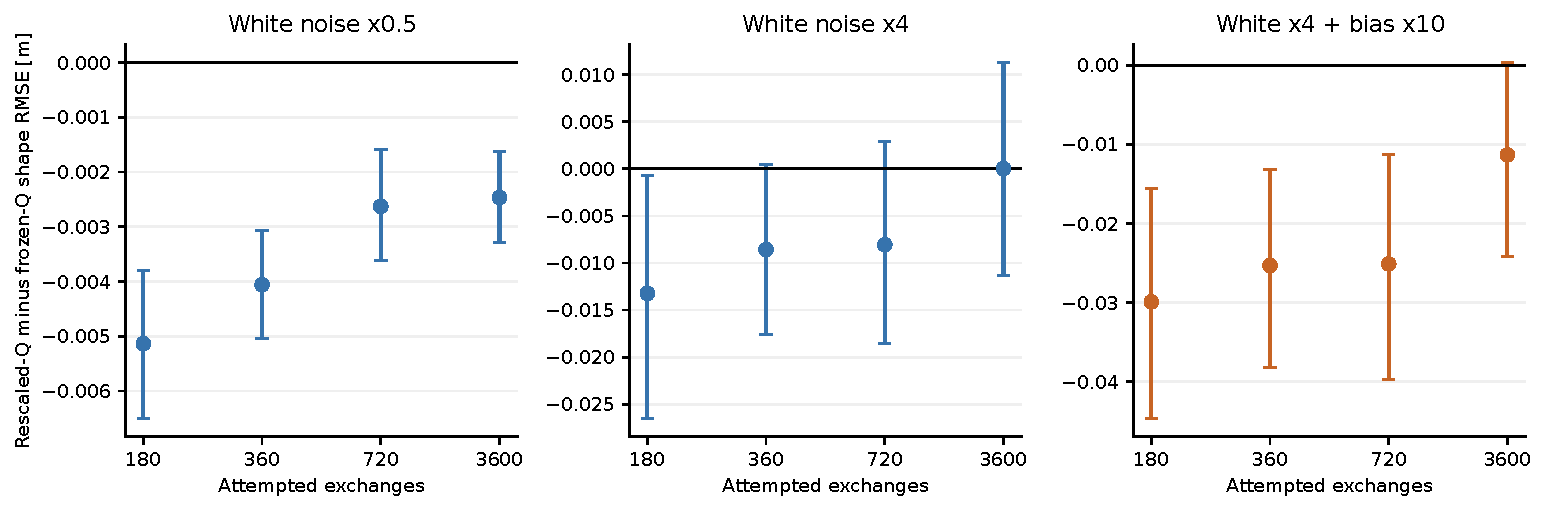
\includegraphics[width=\textwidth]{figures/phase2/p2e_q_adjustment.pdf}
\caption{Rescaled-\(Q\) minus fixed-\(Q\) whole-run shape RMSE with identical sensors and schedules. Markers show paired means and bars show descriptive bootstrap 95\% intervals. Panels use their own vertical scales; interval widths are not raw across-seed RMSE standard deviations. Zero-UWB state differences are exactly zero and omitted.}
\label{fig:p2e_q}
\end{figure}

\begin{table}[htbp]
\centering\small
\caption{Smallest tested budget meeting the predefined \SI{0.10}{m} shape target. Mean and empirical 95th-percentile criteria are separate; ``--'' means not attained even at 3600. Passing seeds are evaluated at the mean-target budget, not at the percentile-target budget.}
\label{tab:p2e_target}
\begin{tabular}{llrrr}
\toprule
Condition & Process covariance & Mean target & 95th percentile & Passing seeds \\
\midrule
Reference & Fixed & 360 & 720 & 18/20 \\
White noise $\times0.5$ & Fixed & 360 & 360 & 19/20 \\
White noise $\times0.5$ & White-rescaled & 180 & 360 & 11/20 \\
White noise $\times4$ & Fixed & -- & -- & -- \\
White noise $\times4$ & White-rescaled & -- & -- & -- \\
Bias drift $\times0.5$ & Fixed & 360 & 360 & 19/20 \\
Bias drift $\times10$ & Fixed & -- & -- & -- \\
White $\times4$, bias $\times10$ & Fixed & -- & -- & -- \\
White $\times4$, bias $\times10$ & White-rescaled & -- & -- & -- \\
\bottomrule
\end{tabular}
\end{table}

Reference and both improved-sensor conditions meet the mean target at 360 exchanges with fixed \(Q\). Fourfold white noise, tenfold bias drift, and combined degradation do not meet it at any tested budget. Neither high-white-noise companion reaches it. Noise-half with rescaled \(Q\) meets the mean at 180 exchanges, \(0.0989\pm0.0160\)~m, compared with reference's smallest passing budget of 360. This is a descriptive half-count result on the tested grid, not a robust 50\% saving: only 11/20 seeds pass at 180 and the empirical 95th percentile is \SI{0.1234}{m}. Its percentile criterion requires 360 exchanges; reference requires 720. These threshold crossings are sensitive to the chosen target and the finite seed set.

\subsection{Time evolution, interpretation, and P2F handoff}
Figure~\ref{fig:p2e_time} shows that degraded sensors retain elevated shape error at both sparse and full communication. Centroid drift grows through the run and is nearly unchanged between those budgets for each condition. Late-window metrics over 40--60 s are retained in the compact results; conclusions use whole-run comparisons, rather than selecting a favorable interval from the curves.
\begin{figure}[htbp]
\centering
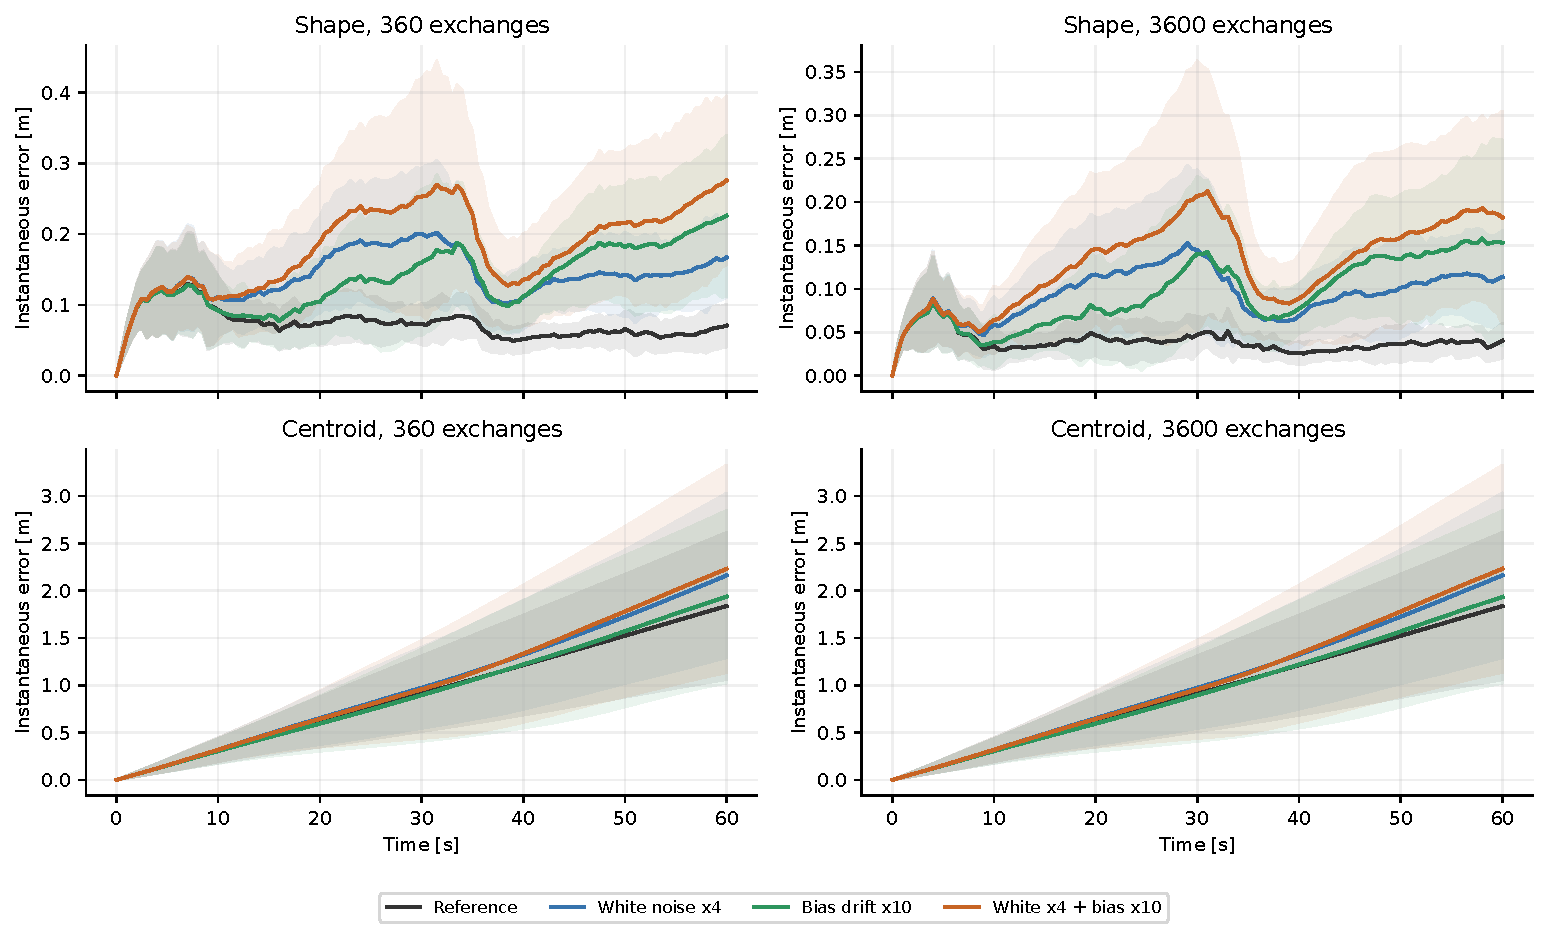
\includegraphics[width=\textwidth]{figures/phase2/p2e_time_profiles.pdf}
\caption{P2E instantaneous shape and centroid error at 360 and 3600 exchanges with fixed \(Q\). Curves show pointwise means and shading mean \(\pm\) one sample standard deviation over 20 seeds, clipped at zero. These are variability bands, not confidence intervals for the means.}
\label{fig:p2e_time}
\end{figure}

P2E establishes that the communication curve depends on IMU noise and bias, and that extra ranges are not an unlimited substitute for sensor quality. It also bounds that conclusion: the primary experiment includes process-noise mismatch, while simple white-noise rescaling helps selectively and leaves bias dynamics unmodeled. The observed floor does not establish an information-theoretic limit or justify a new filter without a separate comparison.

The conditions are stylized amplitude changes on one path set for 60 s. Initial velocity uncertainty is fixed, bias starts at zero, acceleration/gyro levels vary together, and the 10 cm target is descriptive. There are no hardware-derived sensor grades, constant-offset sweeps, longer-duration validation, energy measurements, global references, corruption mixtures, or consistency guarantees. Improved sensors show only modest gains near the existing setting, whereas substantial degradation exposes sensitivity.

Proceed to \textbf{P2F: consolidate the infrastructure-free accuracy--communication frontier}. Keep cyclic as the primary reference and distinguish sensor condition, process-covariance treatment, and P2D range reliability. Relative-shape targets and centroid/absolute-error limits must accompany exchange counts. P2G remains the later optional test of a continuing global reference, and reliability-aware scheduling or bias-state estimation remains a separately justified extension.
\endgroup
